\section{ХОД РАБОТЫ}

\subsection{Постановка задачи}

В ходе данной лабораторной работы требуется выполнить проектирование
и реализацию небольшой экспертной системы с использованием языка Пролог
на основе фреймов.

На основе экспертных оценок (характеристик состояния атомобиля,
водителя и дороги) требуется вычислять подходящую скорость автомобиля.


\subsection{Реализация экспертной системы}

Определим формулу для вычисления скорости автомобиля:
\begin{equation*}
  v = 90 \cdot \sum_{i = 1}^n a_i w_i,
\end{equation*}
где \hspace{2mm} $a_i$ --- оценка ($i$-ого критерия) эксперта, $ a_i \in [0,1] $, \par
$w_i$ --- вес $i$-ого критерия.

Таким образом, для вычисления скорости автомобиля требуется получить оценку
эксперта по трём критериям: состояние дороги, состояние водителя и состояние автомобиля. 

Для упрощения работы эксперта перейдём к словесным характеристикам оценки критерия.
Например, состояние дороги можно оценить как плохое, нормальное или хорошее.

Для каждого из критериев каждой словесной характеристике поставим в соответствие
оценку. Результаты приведены в таблице~\ref{tbl:evals}.
\begin{table}[h!]
  \caption{Соответствие словесных характеристик оценкам.}
  \label{tbl:evals}
  \begin{tabular}{| p{85mm} | c | c | c |}
    \hline
    
    Оценка критерия (состояние) &
    Автомобиль &
    Дорога &
    Водитель \\
    \hline
    
    Плохое      & $0{,}1$ & $0{,}3$ & $0{,}3$ \\ \hline
    Нормальное  & $0{,}5$ & $0{,}5$ & $0{,}5$ \\ \hline
    Хорошое     & $0{,}9$ & $0{,}7$ & $1{,}0$ \\
    \hline
  \end{tabular}
\end{table}

\newpage

Воспользовавшись языком программирования Пролог, создадим
требуемую экспертную систему. Как только эксперт введёт
оценки критериев, а также веса критериев, будет предложена
наиболее благоприятная скорость автомобиля.

Результат работы программы приведен на рисунке~\ref{fig:results}.

\begin{figure}[h!]
  \centering
  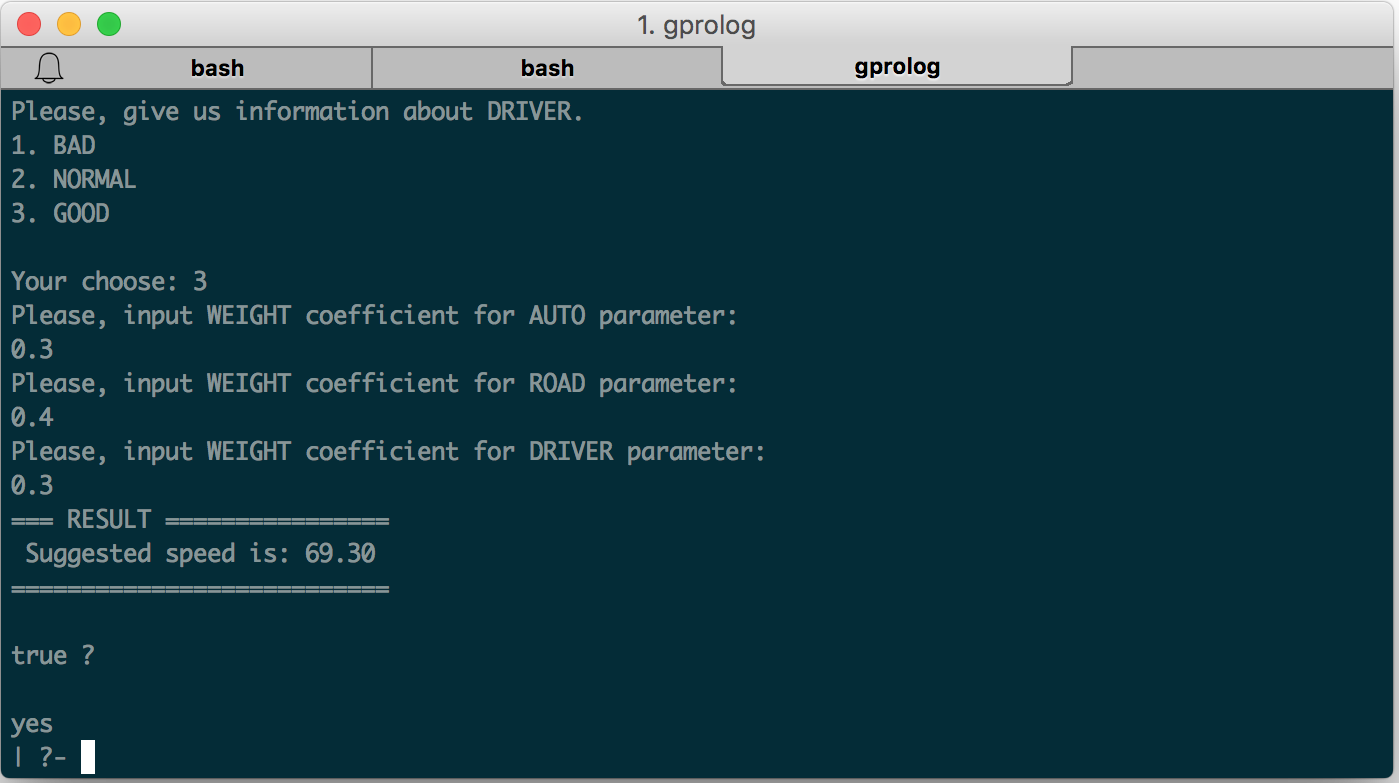
\includegraphics[width=130mm]{img/results}
  \caption{Результат работы программы}
  \label{fig:results}
\end{figure}

Исходный код программы расположен в приложении~А.

\newpage